\documentclass[12pt]{article}

\usepackage{graphicx}
\usepackage[margin=1.0in]{geometry}
\usepackage{amsmath}
\usepackage{cases}
\usepackage{amsfonts}
\usepackage{amssymb}
\usepackage{grffile}
\usepackage{setspace}

\setlength\parindent{0pt}

\author{Xiaohui Chen \\EID: xc2388}
\title{M 362K Pre-Class Work for 2/10}

\begin{document}
\maketitle
\begin{spacing}{2.0}

\section*{3-2}

The distribution is shown below:

\begin{tabular}{|c|c|}
  \hline
  % after \\: \hline or \cline{col1-col2} \cline{col3-col4} ...
  $z$ & $Pr(Z=z)$ \\
  \hline
  1 & 0.1 \\
  \hline
  2 & 0.1 \\
  \hline
  3 & 0.1 \\
  \hline
  4 & 0.1 \\
  \hline
  5 & 0.1 \\
  \hline
  6 & 0.1 \\
  \hline
  7 & 0.1 \\
  \hline
  8 & 0.1 \\
  \hline
  9 & 0.1 \\
  \hline
  10 & 0.1 \\
  \hline
\end{tabular}

\section*{3-3}

\subsection*{(a)}

$Pr(S=1)=\frac{18}{38}$

\subsection*{(b)}

$Pr(S=2)=\left(1-\frac{18}{38}\right)^2*\frac{18}{38}= \frac{900}{6859}$

\subsection*{(c)}
The distribution is shown below:

\begin{tabular}{|c|c|}
  \hline
  % after \\: \hline or \cline{col1-col2} \cline{col3-col4} ...
  $s$ & $Pr(S=s)$ \\
  \hline
  1 & $\frac{18}{38}$ \\
  \hline
  2 & $\left(\frac{20}{38}\right)*\frac{18}{38}$ \\
  \hline
  3 & $\left(\frac{20}{38}\right)^2*\frac{18}{38}$ \\
  \hline
  $\vdots$ & $\vdots$ \\
  \hline
  n & $\left(\frac{20}{38}\right)^{n-1}*\frac{18}{38}$ \\
  \hline
\end{tabular}

\section*{3-5}

\subsection*{(a)}

The probability distribution is shown below:

\begin{tabular}{|c|c|c|c|c|c|c|c|c|c|c|c|}
  \hline
  % after \\: \hline or \cline{col1-col2} \cline{col3-col4} ...
  $s$ & 2 & 3 & 4 & 5 & 6 & 7 & 8 & 9 & 10 & 11 & 12 \\
  \hline
  $Pr(S=s)$ & $\frac{1}{36}$ & $\frac{2}{36}$ & $\frac{3}{36}$ & $\frac{4}{36}$ & $\frac{5}{36}$ & $\frac{6}{36}$ & $\frac{5}{36}$ & $\frac{4}{36}$ & $\frac{3}{36}$ & $\frac{2}{36}$ & $\frac{1}{36}$ \\
  \hline
\end{tabular}

\subsection*{(b)}

The cumulative probability distribution is shown below:

\begin{tabular}{|c|c|c|c|c|c|c|c|c|c|c|c|}
  \hline
  % after \\: \hline or \cline{col1-col2} \cline{col3-col4} ...
  $s$ & 2 & 3 & 4 & 5 & 6 & 7 & 8 & 9 & 10 & 11 & 12 \\
  \hline
  $Pr(S=s)$ & $\frac{1}{36}$ & $\frac{3}{36}$ & $\frac{6}{36}$ & $\frac{10}{36}$ & $\frac{15}{36}$ & $\frac{21}{36}$ & $\frac{26}{36}$ & $\frac{30}{36}$ & $\frac{33}{36}$ & $\frac{35}{36}$ & $\frac{36}{36}$ \\
  \hline
\end{tabular}

\subsection*{(c)}
\begin{figure}
  \centering
  % Requires \usepackage{graphicx}
  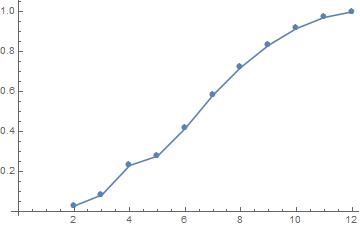
\includegraphics[width=4in]{out1}\\
  \caption{Ogive diagram for S}\label{out1}
\end{figure}

\begin{figure}
  \centering
  % Requires \usepackage{graphicx}
  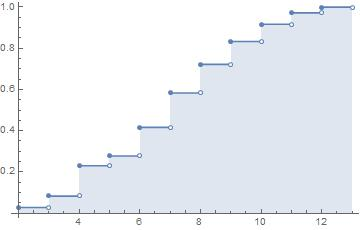
\includegraphics[width=4in]{out2}\\
  \caption{CDF diagram for S}\label{out2}
\end{figure}

The ogive diagram is shown in Figure \ref{out1} and the CDF diagram is shown in Figure \ref{out2}

\end{spacing}
\end{document}